% %%%%%%%%%%%%%%%%%%%%%%%%%%%%%%%%%%%%%%%%%%%%%%%%%%%%%%%%%%%
% Hier nichts aendern
\documentclass[sigconf, nonacm, review]{acmart}
\AtBeginDocument{%
  \providecommand\BibTeX{{%
    \normalfont B\kern-0.5em{\scshape i\kern-0.25em b}\kern-0.8em\TeX}}}

\setcopyright{acmcopyright}
\copyrightyear{2018}
\acmYear{2018}
\acmDOI{XXXXXXX.XXXXXXX}
\acmJournal{JACM}
\acmVolume{37}
\acmNumber{4}
\acmArticle{111}
\acmMonth{8}
\acmPrice{15.00}
\acmISBN{978-1-4503-XXXX-X/18/06}
% Hier nichts aendern
% %%%%%%%%%%%%%%%%%%%%%%%%%%%%%%%%%%%%%%%%%%%%%%%%%%%%%%%%%%%

\begin{document}
% %%%%%%%%%%%%%%%%%%%%%%%%%%%%%%%%%%%%%%%%%%%%%%%%%%%%%%%%%%%
% Hier eigene Daten eingeben
\title{Report zum Fachprojekt Routingalgorithmen}
\author{Ali Almazaal}
\email{ali.almazaal@tu-dortmund.de}

\author{Ahmad Ziadat}
\email{ahmad.ziadat@tu-dortmund.de}



\renewcommand{\shortauthors}{Almazaal, Ziadat,}
% Hier eigene Daten eingeben
% %%%%%%%%%%%%%%%%%%%%%%%%%%%%%%%%%%%%%%%%%%%%%%%%%%%%%%%%%%%

\begin{abstract}
Diese Arbeit wurde während des Kurses "Fachprojekt Routingalgorithmen" an der Fakultät für Informatik an der Technischen Universität Dortmund erstellt. Im Rahmen dieses Projekts haben wir zwei IPv6-Routingalgorithmen entwickelt und erweitert. Unsere Ausarbeitung behandelt die Algorithmen im Detail, einschließlich ihrer Konzepte, Vor- und Nachteile. Unsere Projekte basierten auf dem Paper "Traffic engineering with joint link weight and segment optimization" \cite{foerster2021}. In Projekt 1 haben wir alternative Routingalgorithmen entwickelt und mithilfe der python-basierten Testumgebung des Papers \cite{python-sim} bewertet. Projekt 2 fokussierte sich auf die Evaluierung in Mininet-Experimenten auf Grundlage des Papers\cite{nikolaussuess-nanonet}. Weiterführende Resultate sind über die bereitgestellten Links in den Repositories verfügbar

\end{abstract}

\begin{CCSXML}
<ccs2012>
<concept>
<concept_id>10003033.10003068.10003073.10003076</concept_id>
<concept_desc>Networks~Traffic engineering algorithms</concept_desc>
<concept_significance>500</concept_significance>
</concept>
</ccs2012>
\end{CCSXML}

\ccsdesc[500]{Networks~Traffic engineering algorithms}

% Eventuell keywords weglassen
\keywords{weight optimization, waypoint optimization}



\maketitle

\section{Einleitung}
Traffic Engineering (TE) ist ein grundlegender Aspekt in Netzwerken, der die effiziente Lenkung des Datenverkehrs ermöglicht. Ein innovativer Ansatz namens Segment Routing eröffnet neue Möglichkeiten, den Verkehr intelligent um Engpässe herumzuleiten. Im Gegensatz zu herkömmlichen Methoden, die lediglich Linkgewic-hte anpassen, bietet Segment Routing eine erhöhte Flexibilität. Während die Vorteile dieses Ansatzes bekannt sind, wurde bisher wenig darüber geforscht, wie sich die Optimierung von Linkgewich-ten und Wegpunkten gemeinsam verbessern lässt. Diese Studie untersucht diese dynamische Kombination und beleuchtet, wie sie die Leistung des Netzwerks optimieren kann.\\
Abgesehen von den theoretischen Erkenntnissen präsentieren wir die Ergebnisse unserer Arbeit, die im Rahmen des Bachelor Fachprojekts "Routingalgorithmen" an der Fakultät für Informatik an der Technischen Universität Dortmund entstanden sind. Ziel dieses Projekts war es, Studierende auf reale Forschungsarbeit vorzubereiten und ihnen Einblicke in die Methoden, das Verständnis und die Reproduktion wissenschaftlicher Arbeiten zu vermitteln.\\
Unsere Hauptaufgabe bestand darin, zwei Routingalgorithmen für IPv6-basierte Netzwerke zu entwickeln, basierend auf den Konze-pten der "Greedy-WPO" und "InverseCapacity" Algorithmen, wie sie im Papier "Traffic Engineering with Joint Link Weight and Segment Optimization" \cite{foerster2021} beschrieben sind.\\
In der ersten Projektphase implementierten wir die Algorithmen in Python und unterzogen sie einer eingehenden Prüfung in einer eigens geschaffenen Simulationsumgebung. Hierbei nutzten wir vielfältige Netzwerk-Topologien und simulierte Lastanforderungen für Datenströme. Unsere Tests konzentrierten sich auf die Zielfunktionen "maxMLU", während wir unsere Ergebnisse sorgfältig mit den im genannten Papier beschriebenen Algorithmen verglichen.\\
Die zweite Projektphase involvierte die Anwendung unserer Algorithmen in einer speziell angepassten Version des Netzwerk-Simulationswerkzeugs Nanonet. Durch diese Anwendung führten wir zusätzliche Tests durch und erweiterten die Evaluation unserer Algorithmen, um ihre praktische Anwendbarkeit zu bestätigen.\\
Darüber hinaus haben wir die Projekt 1 und Projekt 2 im Rahmen des 'Fachprojekt-Routingalgorithmen' sowie im Kontext von 'Erweiterte DemandsFirstWaypoints'/'Greedy-WPO'  gründlich überarbeitet und verbessert. Diese aktualisierten Ausführungen habe ich in einem neuen Repository hochgeladen\cite{new-repo}.
\section{Theoretische Grundlagen}

{Unsere Forschung baut auf der Arbeit von Mahmoud Parham, Thomas Fenz, Nikolaus Süss, Klaus-Tycho Foerster und Stefan Schmid auf, die in ihrem Paper "Traffic Engineering with Joint Link Weight and Segment Optimization" \cite{foerster2021}. eine innovative Methode zur Verbesserung der Internet-Traffic-Routing präsentierten. Diese Methode beinhaltet die Verwendung von Wegpunkten, welche von der üblichen Praxis abweicht, den Traffic über die kürzesten Wege zu leiten. Stattdessen werden Zwischenziele eingefügt, durch die eine Nachfrage passieren muss. Dies ermöglicht eine Entlastung überlasteter Netzwerkknoten, die sich auf frequentierten kürzesten Pfaden befinden, wenn die Auswahl der Wegpunkte entsprechend erfolgt. Dadurch wird die angestrebte Zielfunktion weniger stark beeinträchtigt. Darüber hinaus wird die herkömmliche Methode der Routingalgorithmen, die den kürzesten Pfad verwenden, mit der Idee der Wegpunkte im Joint Algorithmus kombiniert. Dieser Joint Algorithmus wird im besagten Paper ausführlich bewertet und analysiert.}
\subsection{DemandsFirstWaypoints}
\label{sec:1}
{Die "DemandsFirstWaypoints"-Klasse präsentiert einen fortschrittlichen Algorithmus zur Lösung des Routenplanungsproblems in Netzwerken. Dieser Algorithmus kombiniert Graphentheorie, Optimierung und Algorithmik, um optimale oder nahezu optimale Routen zu identifizieren und gleichzeitig die Auslastung des Netzwerks zu minimieren. Er betrachtet die Netzwerktopologie als einen Graphen, in dem Knoten Standorte und Kanten Verbindungen sind. Die Kapazitäten der Kanten geben an, wie viel Datenverkehr sie tragen können. Der  Algorithmus legt den Schwerpunkt auf die Auswahl von Zwischenzielen für Nachfragen, um die Lastverteilung in einem Netzwerk zu optimieren. Er verwendet eine iterative Methode, um für jedes Nachfragepaar alle Knoten als potenzielle Zwischenziele zu betrachten. Anschließend wird überprüft, ob die Einbeziehung eines bestimmten Zwischenziels zu einer besseren Lastverteilung und Netzwerknutzung führt. Diese innovative Lösung findet Anwendung in verschiedenen Bereichen wie Logistik, Telekommunikation und Verkehrsmanagement, wo die effiziente Nutzung von Netzwerkressourcen und die Erfüllung der Nachfrage von entscheidender Bedeutung sind.}
\subsection{InverseCapacity}
die "Inverse Capacity" aus dem Papier \cite{foerster2021} ist, ein effizientes Verfahren zur Lösung eines Netzwerkoptimierungsproblems zu implementieren. Dabei wird die Wahl der optimalen Pfade in einem Netzwerk durch die Verwendung von inversen Kapazitäten gesteuert, um Engpässe zu minimieren. Der Code implementiert eine Methode zur Gewichtung der Netzwerkverbindungen basierend auf inversen Kapazitäten und nutzt anschließend den "EqualSplitShortestPath"-Algorithmus, um die besten Pfade für gegebene Anforderungen zu finden. Das Ergebnis umfasst neben den optimalen Pfaden auch Informationen zur Ausführungszeit des Algorithmus.

\section{REPLIKATION}
{Die Praxis der wissenschaftlichen Replikation bietet eine wertvolle Gelegenheit zur Verifizierung experimenteller Ergebnisse, wodurch die Zuverlässigkeit dieser Resultate bestätigt werden kann. In unserem Fall eröffnete sich die Möglichkeit, sowohl die Resultate der zugrunde liegenden Studie als auch die Ergebnisse einer anderen Forschungsgruppe zu überprüfen. Diese Replikation zwischen den Forschungsgruppen legt besonderen Fokus auf die Schaffung von Nachvollziehbarkeit und trägt dazu bei, die Glaubwürdigkeit der experimentellen Befunde zu stärken. Letztendlich stellt die Replikation eine essentielle Grundlage dar, um Vertrauen in die erzielten Forschungsergebnisse aufzubauen.}

\subsection{Replikation Gruppe 1}
{Unsere nächsten Schritte beinhalten die Reproduktion der Methodik von Gruppe 1, begleitet von der Präsentation beispielhafter Daten zur Überprüfung durch den Leser.}
\subsubsection{Replikation zu Projekt 1}
{Die Replikation dieses Projekts \cite{replication-group1-pro1} verlief reibungslos, da die Gruppe ihr Repository so vorbereitet hatte, dass eine direkte Bewertung des Projekts möglich war, vorausgesetzt, der Nutzer hatte die erforderlichen Abhängigkeiten installiert. Nach einer gewissen Rechenzeit konnten die Ergebnisse problemlos mithilfe des mitgelieferten Plotters visualisiert werden. Unsere eigenen Resultate stimmen mit den Daten der Gruppe überein, was uns in die Lage versetzt, die Reproduzierbarkeit des ersten Experiments durch die Gruppe zu bestätigen.}

\begin{figure}
\centering
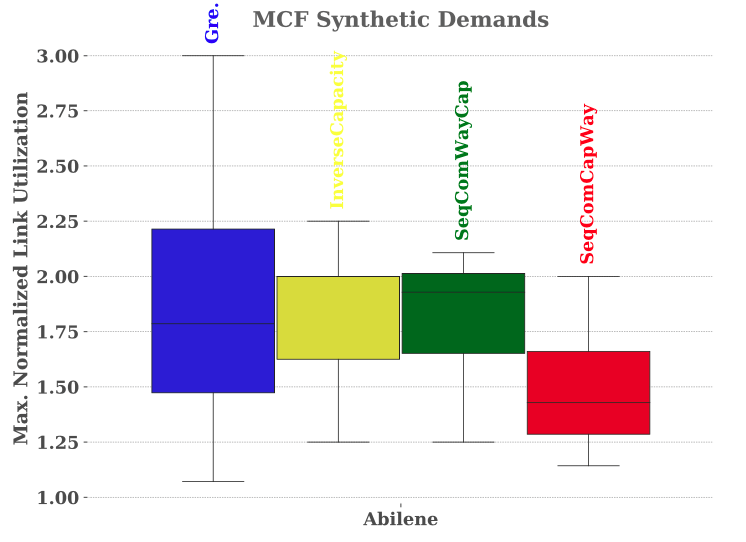
\includegraphics[width=\linewidth]{figures/p.png}
\caption{Beispielplot aus der Replikation der Gruppe 1.}
\label{fi}
\end{figure}

\begin{figure}
\centering
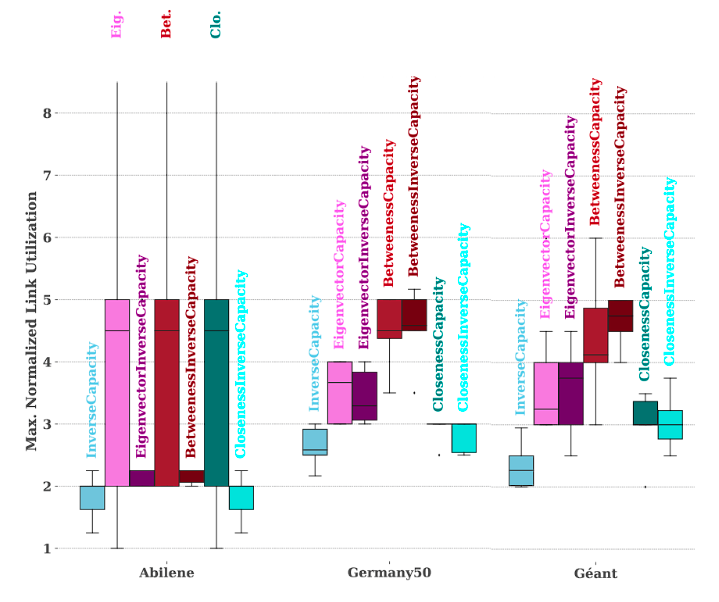
\includegraphics[width=\linewidth]{figures/k.png}
\caption{Beispielplot aus der Replikation der Gruppe 1.}
\label{fi1}
\end{figure}

\subsubsection{Replikation zu Projekt 2}
{Auch das zweite Projekt \cite{replication-group1-pro2} der anderen Gruppe nahm die Grundideen von Projekt 1 auf und setzte diese in Form von Experimenten mit Nanonet um. Die Replikation des Codes der Gruppe verlief insgesamt reibungslos. Während der Ausführung des Codes traten keinerlei Probleme auf, sofern sämtliche benötigten Abhängigkeiten korrekt installiert waren. Unsere eigenen Resultate stimmen weitgehend mit den Daten der Gruppe überein, was die Nachvollziehbarkeit ihrer Ergebnisse bekräftigt.\\
Eine Herausforderung, der wir innerhalb unserer eigenen Gruppe begegneten, war das direkte Vergleichen der Verläufe, obwohl sie für unterschiedliche Topologien und Anforderungen simuliert wurden. Dies unterstreicht die Notwendigkeit, die Kontextunterschiede zu berücksichtigen, um angemessene Schlussfolgerungen aus den Vergleichen zu ziehen.}

\begin{figure}
\centering
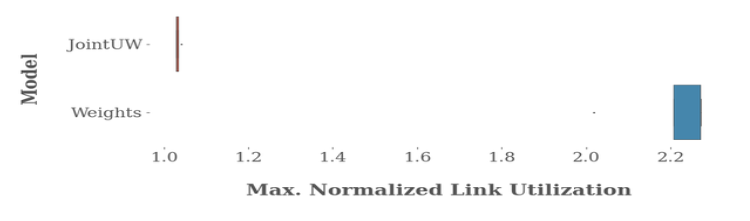
\includegraphics[width=\linewidth]{figures/n1.png}
\caption{Beispielplot aus der Replikation der Gruppe 1.}
\label{fi2}
\end{figure}

\begin{figure}
\centering
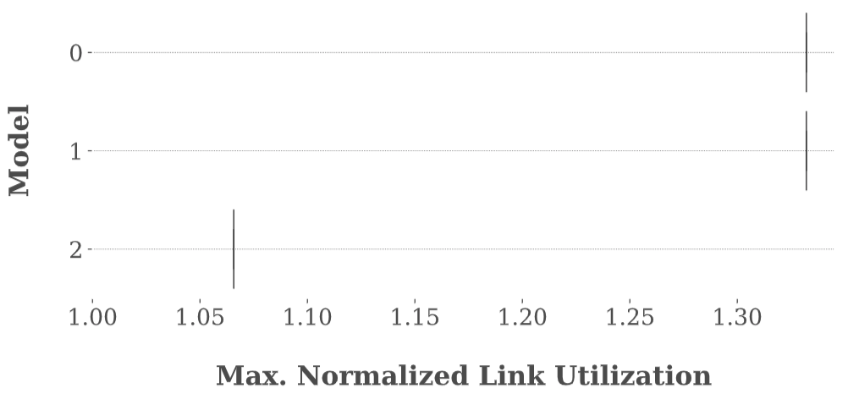
\includegraphics[width=\linewidth]{figures/p1.png}
\caption{Beispielplot aus der Replikation der Gruppe 1.}
\label{fi3}
\end{figure}


\section{UNSERE EIGENEN ALGORITHMEN}
\subsection{Resultate zu Projekt 1}

\subsubsection{Erweiterte DemandsFirstWaypoints }
Unser erster Algorithmus trägt den Namen 'Erweiterte DemandsFirstWaypoints' und stellt eine modifizierte Ableitung des 'DemandFirstWaypoints'-Algorithmus dar. Eine kurze Beschreibung dieses Algorithmus findet sich im Bericht unter dem Abschnitt \ref{sec:1} und wird im Detail im Paper \cite{foerster2021} erläutert.\\
Das Ziel dieser Arbeit bestand darin, sowohl die Effizienz als auch die Effektivität des Algorithmus zur Minimierung der Maximallastunterschiede (MLU) zu erhöhen. Hierfür wurde die Methode \_\_demands\_first\_waypoints durch entscheidende Verbesserungen erweitert, um die Leistungsfähigkeit des Algorithmus zu maximieren.\\
Die optimierte Methode führt verschiedene innovative Verbesserungen ein, um die Effizienz und Genauigkeit der Wegpunktauswahl zu erhöhen:\\
\textbf{Innovative Wegpunktauswahl:}
Eine der zentralen Neuerungen dieser optimierten Methode liegt in der verfeinerten Auswahl potenzieller Wegpunkte. Im Code wurden die Top-K benachbarten Knoten entlang des kürzesten Pfades, welche die höchsten Kapazitäten aufweisen, als mögliche Wegpunkte ausgewählt. Diese innovative Idee zielt darauf ab, die Anzahl der in Betracht gezogenen Knoten als mögliche Wegpunkte für eine bestimmte Nachfrage (Demand) zu beschränken. Dies hat das Ziel, die Laufzeit des Algorithmus zu reduzieren.\\
\textbf{Kürzeste Pfade-Cache:} Eine weitere signifikante Verbesserung besteht in der Einführung eines Caches für bereits berechnete kürzeste Pfade zwischen Knotenpaaren. Dies ermöglicht die Wiederverwendung von Ergebnissen und reduziert die Notwendigkeit aufwändiger Neuberechnungen.\\
\textbf{Mögliches Waypoints-Set:}  Die Methode generiert ein Set von potenziellen Wegpunkten entlang der kürzesten Pfade, indem sie die Kapazitäten der benachbarten Knoten berücksichtigt. Dabei wählt sie die Top-Nachbarn mit den höchsten Kapazitäten aus. Diese präzise Auswahl reduziert die Anzahl der Optionen.\\
In Ergänzung zu diesen Verbesserungen wurden auch andere Faktoren und Metriken einzeln wie die verfügbaren Kapazitäten und die Auslastung der benachbarten Knoten entlang der kürzesten Pfade in Betracht gezogen, um die Effizienz und Lösungsqualität des Algorithmus weiter zu optimieren.\\
\begin{figure}
\centering
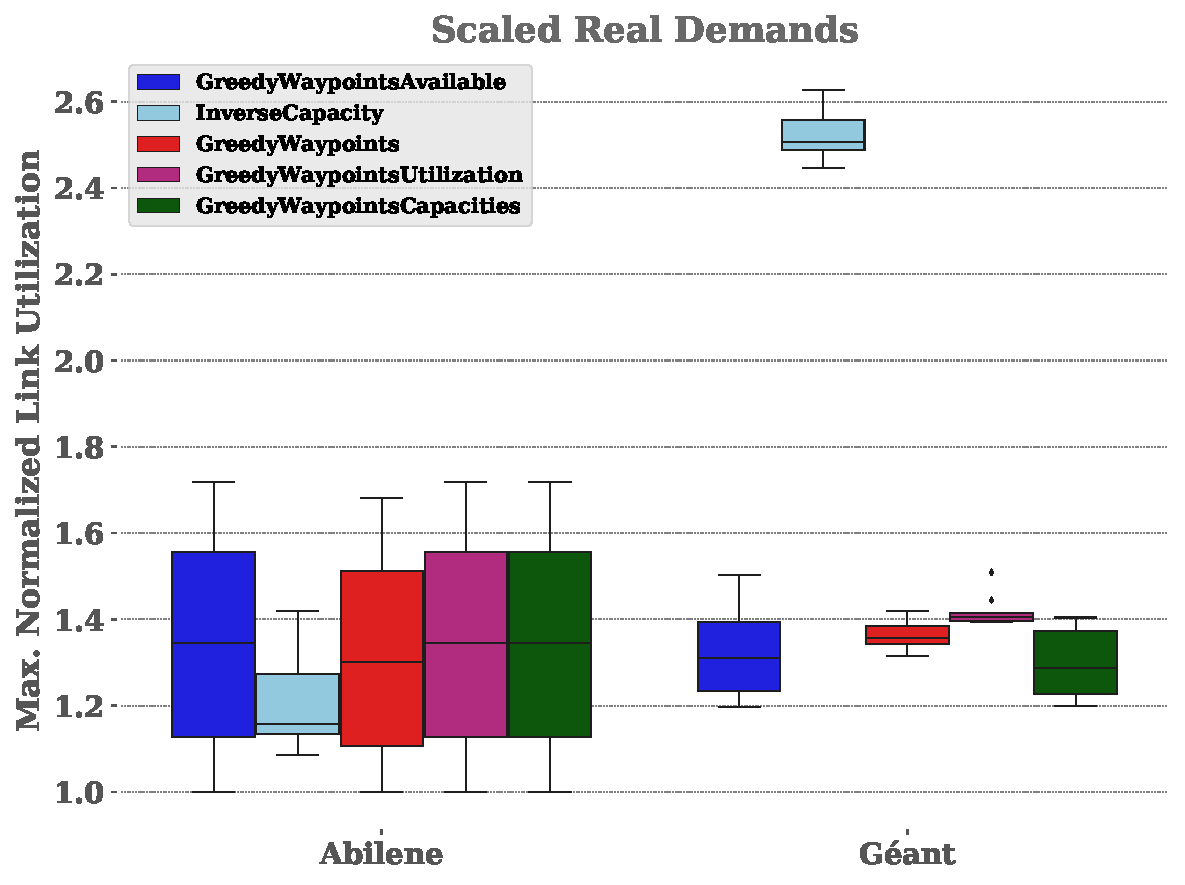
\includegraphics[width=\linewidth]{figures/real_demands.pdf}
\caption{Vergleich von fünf Algorithmen mit Realen Anforderungen auf der Abilene- und Geant-Topologie.\emph{"GreedyWaypointsCapacities" stellt die erweiterte Version von "DemandsFirstWaypoints" in darkgreen dar."GreedyWaypointsAvailable" stellt die Berücksichtigung der verfügbaren Kapazitäten der benachbarten
Knoten in blau dar."GreedyWaypointsUtilization" stellt die Berücksichtigung der Auslastung der benachbarten Knoten in mediumVioletred }}
\label{fig}
\end{figure}
\textcolor{blue}{Berücksichtigung der verfügbaren Kapazitätender benachbarten Knoten:} Die Erweiterung der Methode beinhaltet eine intelligente Auswahl potenzieller Wegpunkte auf Grundlage der verfügbaren Kapazitäten der benachbarten Knoten.\\
\textcolor{violet} {Berücksichtigung der Auslastung der benachbarten Knoten:} In
der erweiterten Methode werden potenzielle Wegpunkte basierend
auf den Top-k benachbarten Knoten mit der niedrigsten Auslastung
entlang der kürzesten Pfade ausgewählt.\\

\begin{figure}
\centering
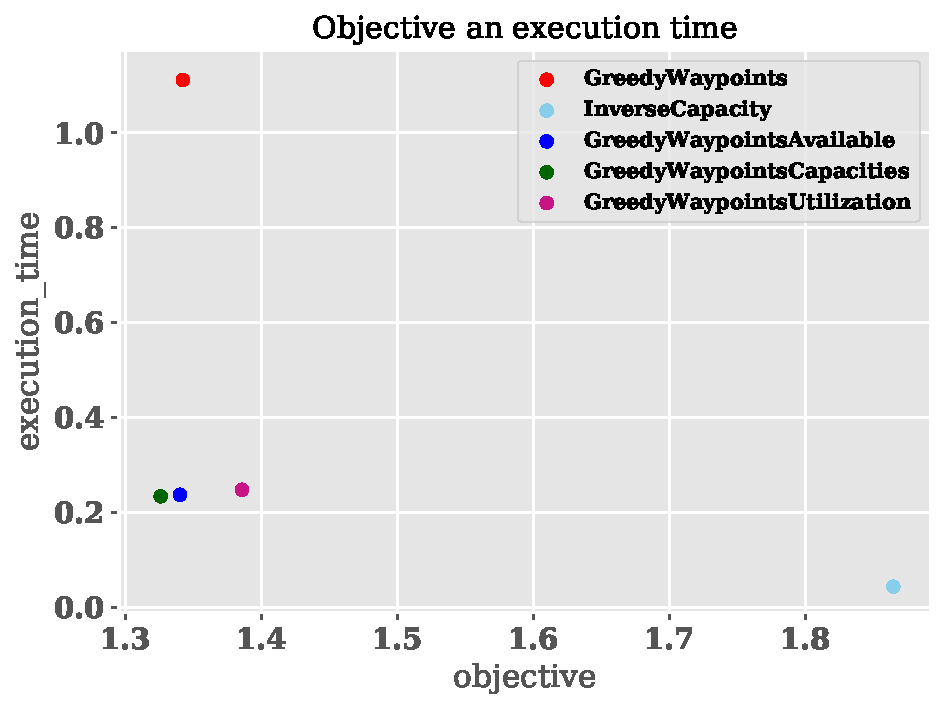
\includegraphics[width=\linewidth]{figures/execution_time.pdf}
\caption{Vergleich von fünf Algorithmen mit Realen Anforderungen auf der Abilene- und Geant-Topologie.\emph{"GreedyWaypointsCapacities" stellt die erweiterte Version von "DemandsFirstWaypoints" in darkgreen dar.}}
\label{fig1}
\end{figure}
Die oben beschriebenen Ansätze wurden sorgfältig untersucht und in umfangreichen Tests mit der erweiterten Methode verglichen wie in die Abbildungen \ref{fig} \ref{fig1}. Die Ergebnisse zeigen, dass die Berücksichtigung der verfügbaren Kapazitäten und der Auslastung der benachbarten Knoten zwar interessante Ansätze sind, jedoch im Vergleich zur optimierten Methode leicht schlechtere Ergebnisse lieferten. Die Kombination dieser Faktoren kann in bestimmten Szenarien möglicherweise zu einer geringfügigen Verschlechterung der Lösungsqualität führen. Daher wurde in der finalen Version der optimierten Methode die Auswahl der Top-K benachbarten Knoten mit den höchsten Kapazitäten entlang des kürzesten Pfades als effektivste Option ausgewählt, um die gewünschten Ergebnisse zu erzielen.\\
\textbf{Vorteile und Auswirkungen:}\\
Die optimierte Methode bietet mehrere Vorteile im Vergleich zur ursprünglichen Version:\\
Effiziente Berechnungen: Die Nutzung des Cache für kürzeste Pfade sowie die präzise Auswahl von Top-Nachbarn reduzieren die Berechnungszeit erheblich. Dadurch beschleunigt sich die Gesamtausführung des Algorithmus.\\
Relevante Wegpunkte: Die Methode konzentriert sich bei der Auswahl potenzieller Wegpunkte auf Knoten, die aufgrund ihrer Kapazität die optimale Lastverteilung ermöglichen. Dadurch steigt die Wahrscheinlichkeit, optimale Lösungen zu finden.\\
Anpassungsfähigkeit: Die Möglichkeit zur Anpassung der Anzahl der Top-Nachbarn ermöglicht eine gezielte Feinabstimmung des Algorithmus auf verschiedene Netzwerkkonfigurationen und Anforderungen.\\
\textbf{Ansatzklassifizierung:}\\
Die optimierte Methode lässt sich in verschiedene Ansatzkategorien einordnen:\\
Heuristische Auswahl: Durch die Auswahl von vielversprechenden Wegpunkten mithilfe von Kriterien wie Kapazität und Top-Nachbarn nutzt die Methode eine heuristische Strategie. Dies optimiert den Lösungsraum und reduziert die Suche nach optimalen Lösungen.\\
Berücksichtigung der Netzwerktopologie: Die Methode nutzt die Netzwerktopologie, um kluge Wegpunkte zu identifizieren. Dabei fokussiert sie sich auf Knoten mit höheren Kapazitäten, um die Effizienz der Lastverteilungsoptimierung zu maximieren.\\
Es ist wichtig zu beachten, dass die Methode auch Elemente aus anderen Ansätzen enthält:\\
Lokale Suche durch heuristische Auswahl: Die Auswahl der Top-K benachbarten Knoten ähnelt einer "lokalen Suche". Dies fokussiert die Aufmerksamkeit auf wenige potenzielle Wegpunkte, um bessere Lösungen zu erzielen.\\
Dynamische Anpassung: Die Optimierung der Wegpunktauswahl kann als Form der "Dynamischen Anpassung" betrachtet werden. Sie reagiert während der Laufzeit auf neue Informationen, um den Flussverkehr umzuleiten und die MLU zu minimieren.\\
\textbf{Schlussfolgerung:}\\
Die erweiterte Methode \_\_demands\_first\_waypoints stellt eine signifikante Weiterentwicklung dar, die auf intelligenten Algorithmen basiert, um die Wegpunktauswahl zu optimieren. Durch die Integration von kürzesten Pfaden, Berücksichtigung der benachbarten Knotenkapazitäten und Nutzung des Dijkstra-Algorithmus werden erhebliche Verbesserungen in Effizienz und Lösungsqualität erzielt.\\
In Tests haben wir festgestellt, dass die modifizierte Methode die Berechnungseffizienz im Vergleich zur ursprünglichen Methode verbessert. Allerdings gibt es einen Kompromiss - die maximale Auslastung kann je nach Topologie variieren. In einigen Fällen war die modifizierte Methode besser, in anderen war sie schlechter.


\subsubsection{Erweiterte Inverse Capacity} 
Die effiziente Nutzung von 
Resso-urcen in modernen Netzwerken und die Steigerung ihrer Leistung sind essenziell, um den wachsenden Anforderungen gerecht zu werden. Unser zweiter Algorithmus nennt sich 'Erweiterte Inverse Capacity' und ist eine Erweiterung des 'inverse Capacity' aus dem Paper \cite{foerster2021}. Die vorgestellte Methode nutzt die Gewichtung von Verbindungen im Netzwerk, indem die Gewichte entsprechend ihrer Kapazität umgekehrt werden. Dies ermöglicht eine präzisere Routenauswahl und verbesserte Ressourcennutzung. Hintergründig bestimmt die Kapazität einer Verbindung die maximale Datenmenge, die sie übertragen kann. Die Routenplanung basiert oft auf dem Dijkstra-Algorithmus, der kürzeste Pfade ermittelt. Ziel dieses Projekts ist es, diesen Prozess zu optimieren, indem die inverse Kapazität genutzt wird.
\begin{figure}[h]
\centering
{\hspace{+6cm}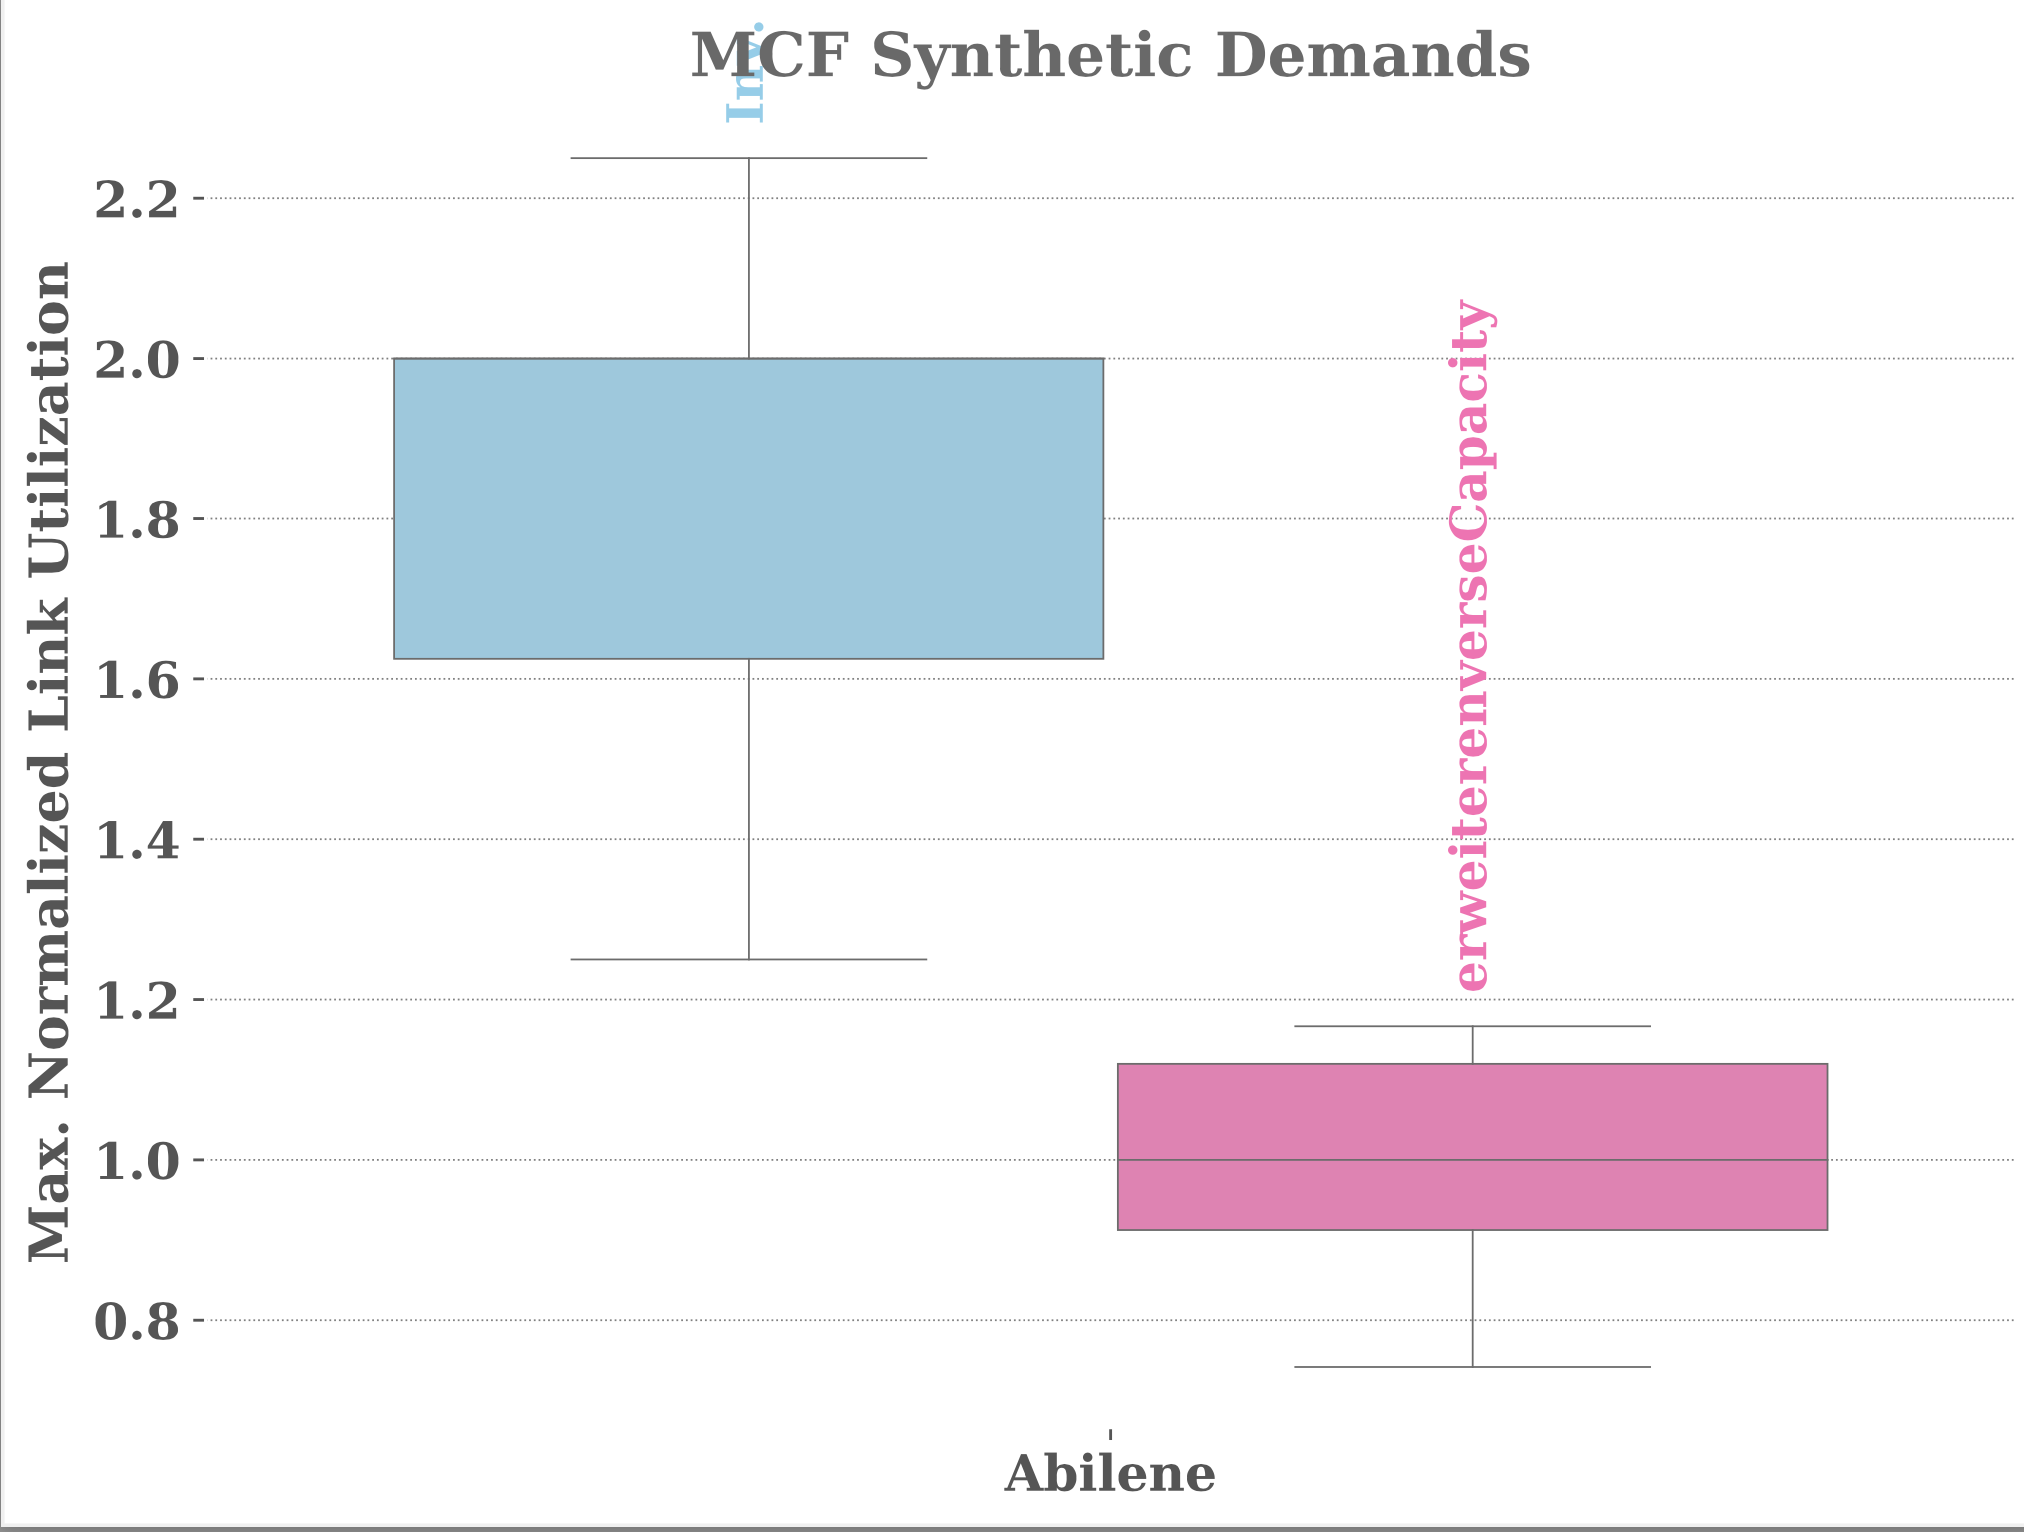
\includegraphics[width=0.4\textwidth]{a4.png}} 
\caption{Vergleich die inverse capacity mit die Erweiterte Inverse Capacity auf der Abilene-Topologie. Legende: \emph{inverse capacity} in skyblue, \emph{Erweiterte Inverse Capacity} in hotpink.}
\label{fig:1}
\end{figure}
Der entwickelte Algorithmus basiert auf dieser Methode und kehrt die Gewichtungen der Verbindungen um. Dadurch präferiert der Dijkstra-Algorithmus Wege mit höherer Kapazität, was zu schnelleren und effizienteren Verbindungen führt. Zusätzlich zur Berechnung des kürzesten Pfads identifiziert der Algorithmus alternative Routen, indem der kürzeste Pfad umgekehrt wird, um überlasteten Verbindungen auszuweichen. Die Bewertung der Link-Auslastung erfolgt mithilfe einer Funktion, die die aktuelle Auslastung basierend auf Anfragen berechnet. Eine maximale Auslastungsschwelle dient der Vermeidung von Überlastungen. Wenn ein Link diese Schwelle überschreitet, greift der Algorithmus auf alternative Maßnahmen wie die Nutzung von Ersatzrouten oder Notfallstrategien zurück. Die Implementierung nutzt die NetworkX-Bibliothek in Verbindung mit dem Dijkstra-Algorithmus, was eine effiziente Umsetzung des inversen Kapazitätsalgorithmus zur Routenoptimierung ermöglicht. Die Leistung des Algorithmus wurde mittels verschiedener Metriken, einschließlich Verbindungsbelastung und Effizienz der gewählten Routen, bewertet. Die Ergebnisse in den Abbildungen 1 und 2 zeigen eine bedeutende Verbesserung der Netzwerkleistung im Vergleich zu herkömmlichen Ansätzen. Zusammenfassend stellt der entwickelte Ansatz eine wirkungsvolle Methode zur Netzwerkleistungsoptimierung dar.

Die Umkehrung der Gewichtungen basierend auf der Kapazität führt zu einer verbesserten Routenauswahl und effizienteren Ressourcennutzung. Die vielfältigen Anwendungsmöglichkeiten dieses Ansatzes eröffnen neue Potenziale zur Steigerung der Netzwerkeffizienz in verschiedenen Umgebungen. Zukünftige Entwicklungen könnten eine noch genauere Anpassung des Algorithmus an spezifische Netzwerkanforderungen beinhalten, um seine Wirksamkeit weiter zu erhöhen.

\begin{figure}
\centering
{\hspace{+6cm}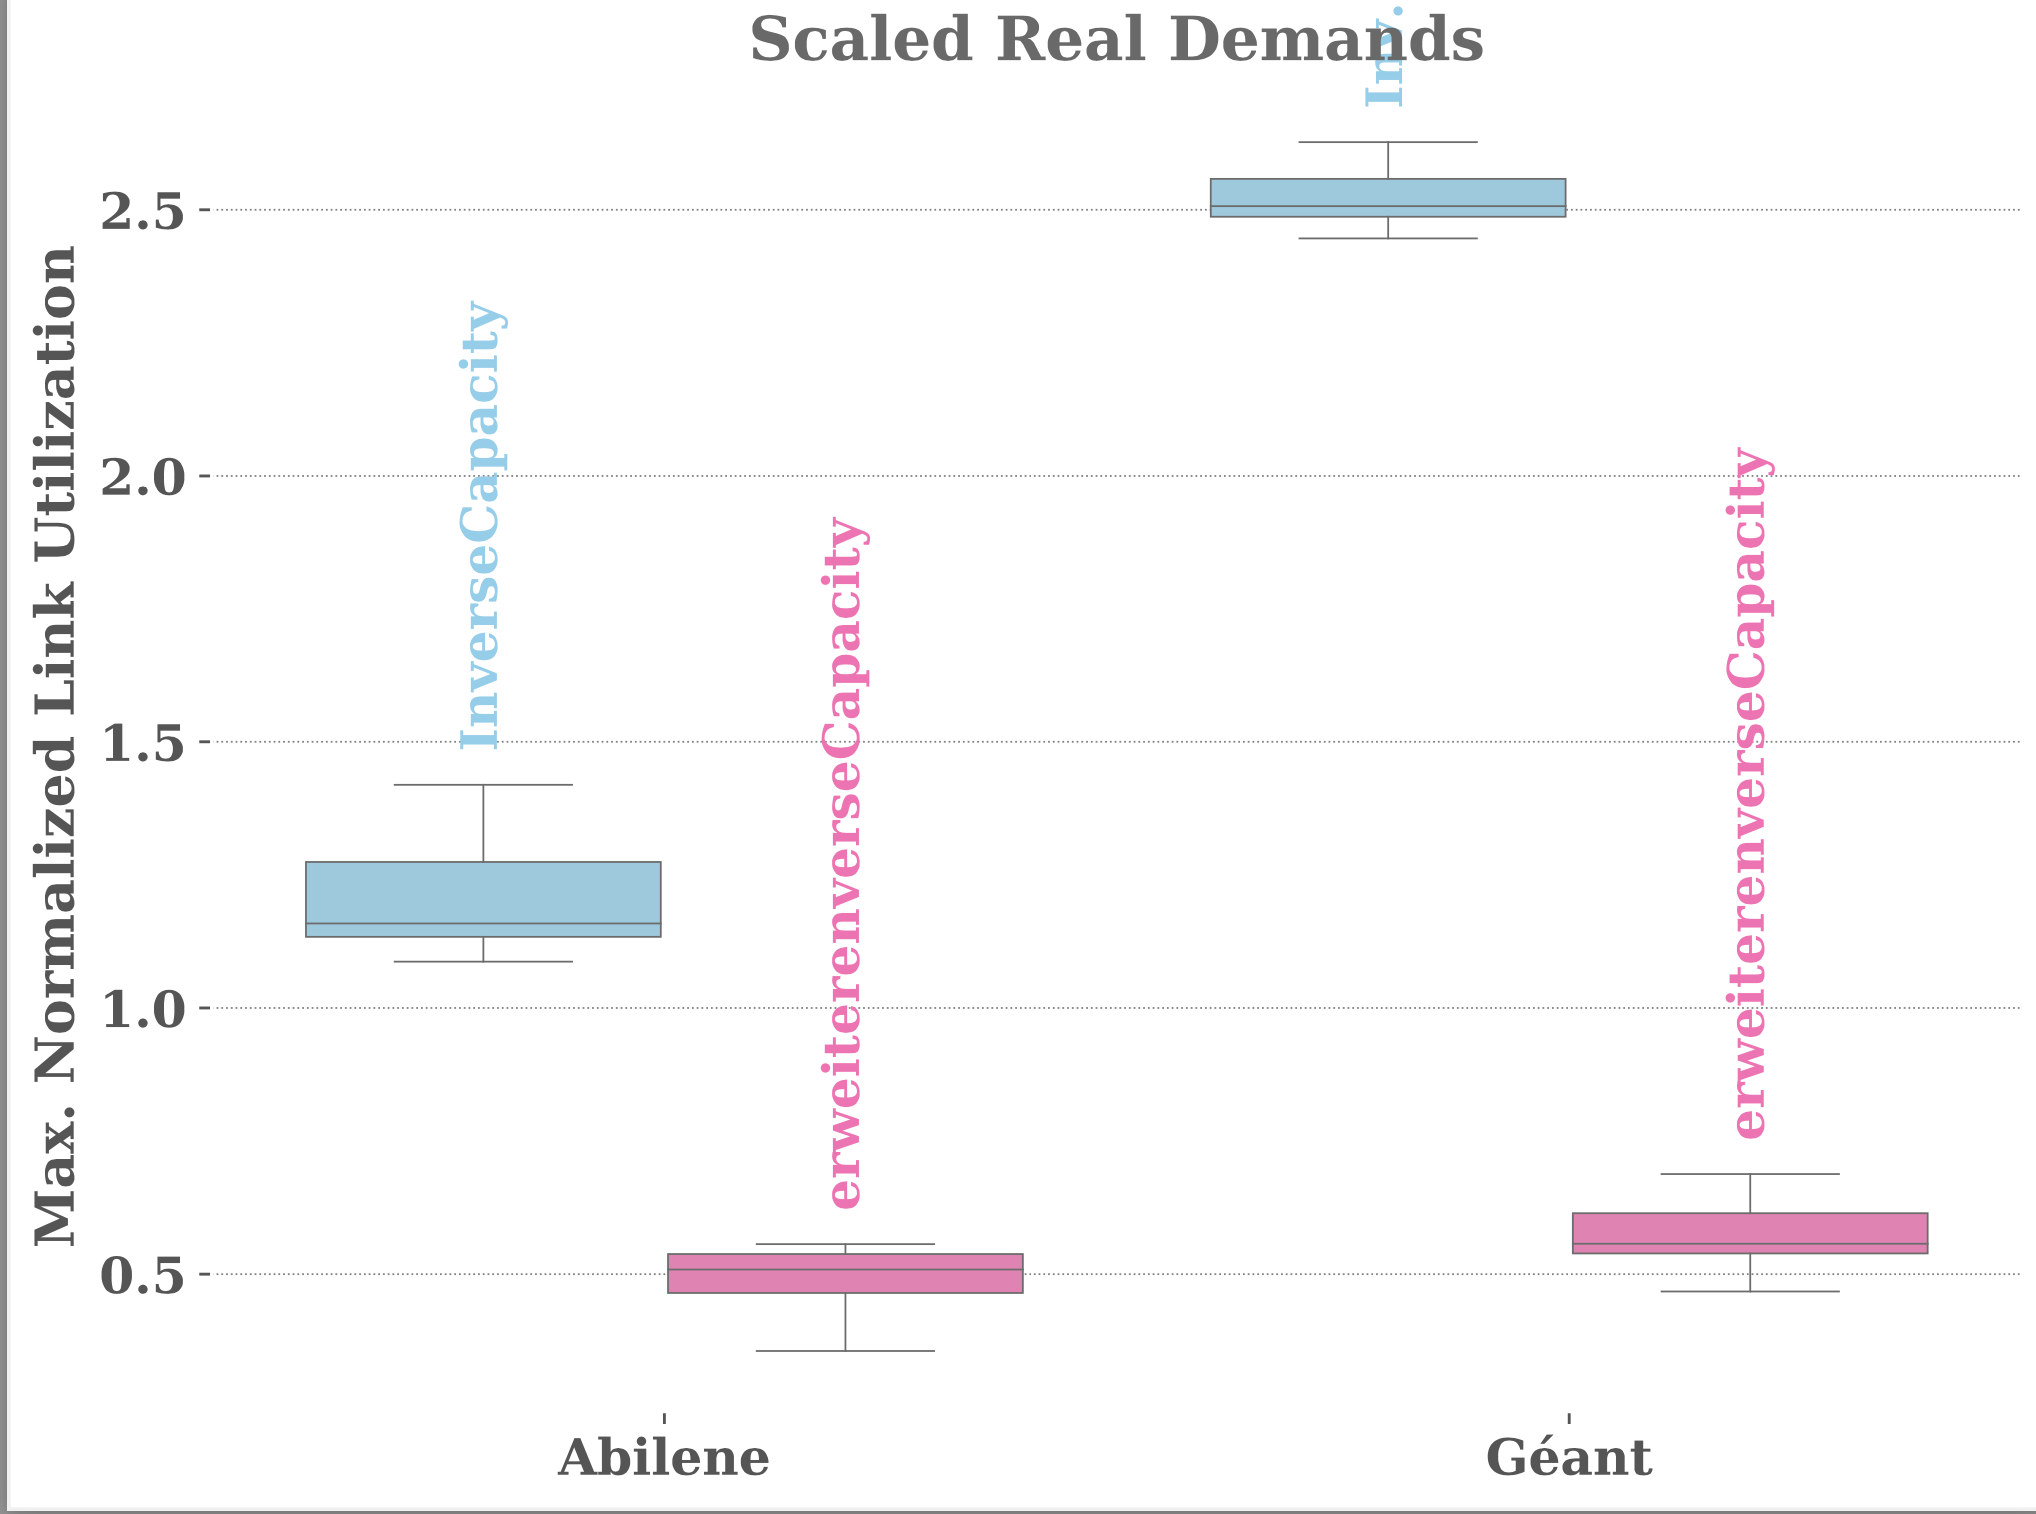
\includegraphics[width=0.4\textwidth]{a5.png}} 
\caption{Vergleich die inverse capacity mit die Erweiterte Inverse Capacity auf verschiedne-Topologie in Real Demands  . Legende: \emph{inverse capacity} in skyblue, \emph{Erweiterte Inverse Capacity} in hotpink.}
\label{fig:11}
\end{figure}

\subsection{Resultate zu Projekt 2}
Die zweite Reihe von Experimenten baut ebenfalls auf dem genannten Papier auf, doch lag hier nicht der Hauptfokus auf der Python-Implementierung. Vielmehr hatten wir das Ziel, unsere Modifikationen aus Projekt 1 unter realistischen Bedingungen zu überprüfen. Für die Simulation des Netzwerks kamen keine physischen Hardwarekomponenten zum Einsatz. Stattdessen nutzten wir ein in Nanonet integriertes Simulationsframework \cite{nanonet} \cite{nikolaussuess-nanonet}, um im Linux-Kernel eine authentische Netzwerkumgebung nachzubilden. Dies ermöglichte es uns, das Verhalten der Algorithmen unter realen Bedingungen zu testen. Zusätzlich strebten wir an, unsere Konzepte durch angemessene Skalierung bestmöglich zu verdeutlichen.\\
\\
\textbf{ Erweiterte Inverse Capacity} \\
das Test des erweiterte Inverse Capacity Algorithmus beschreibt eine Kommunikationsinfrastruktur zwischen verschiedenen Knoten. Eine einzige Nachfrage besteht von Knoten 0 zu Knoten 4, wobei Daten im Umfang von 4 Einheiten übertragen werden sollen. Es besteht eine interessante Möglichkeit, einen Wegpunkt bei Knoten 4 mit einer Wahrscheinlichkeit von 50 prozent zu nutzen. Dies bedeutet, dass die Datenübertragung den vorgesehenen Wegpunkt in Erwägung zieht, was Flexibilität und Optimierung der Übertragung ermöglicht.
Die Knoten sind durch eine Anzahl von Links miteinander verbunden. Jeder Link repräsentiert eine Verbindung zwischen zwei Knoten und hat eine Kapazität, die angibt, wie viele Daten gleichzeitig übertragen werden können. Diese Kapazitäten variieren zwischen den Links, wobei einige Verbindungen mehr Daten gleichzeitig übertragen können als andere.
Die maximale Link-Auslastungsschwelle von 2.0 dient als Leitlinie, um sicherzustellen, dass die Verbindungen nicht überlastet werden. Dies bedeutet, dass die Datenübertragung auf den Links so verteilt werden soll, dass die Auslastung jedes Links diese Schwelle nicht überschreitet. Dieses Ziel ist wichtig, um eine reibungslose und effiziente Kommunikation innerhalb der Infrastruktur sicherzustellen.
Der zugrunde liegende Algorithmus basiert auf dem "Inverse Capacity" Ansatz und optimiert die Routenwahl unter Berücksichtigung der umgekehrten Kapazität der Verbindungen. Darüber hinaus berücksichtigt der Algorithmus alternative Routen, um sicherzustellen, dass die Link-Auslastung stets innerhalb der festgelegten Schwelle bleibt.
Insgesamt zielt dieser Algorithmus darauf ab, eine effiziente und zuverlässige Datenübertragung in der gegebenen Infrastruktur zu gewährleisten, indem er sowohl die Kapazität der Verbindungen als auch die Auslastung der Links berücksichtigt.
\begin{figure}[h]
\centering
{\hspace{+6cm}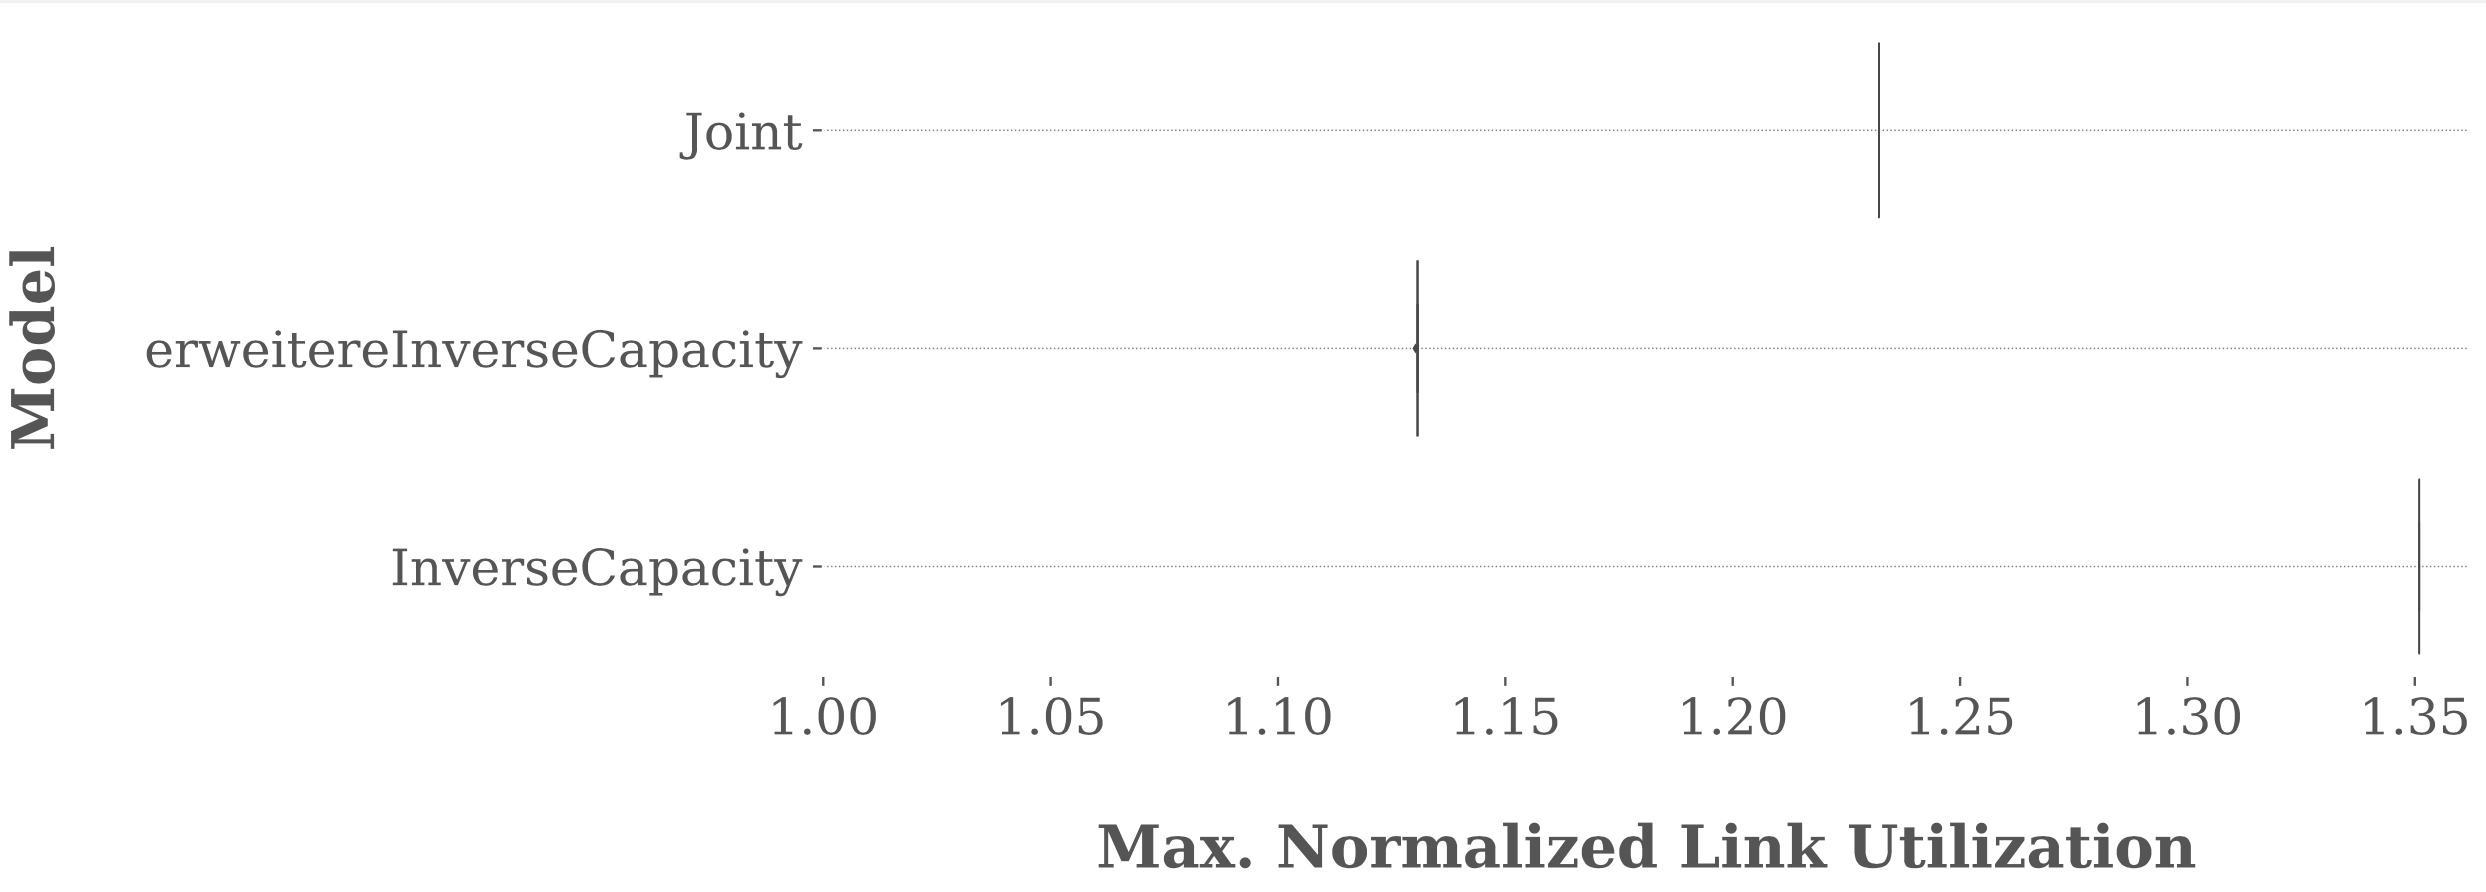
\includegraphics[width=0.5\textwidth]{a6.png}} 
\caption{ Ergebnisse für die Erweiterte Inverse Capacit mit inverse capacity} 
\label{fig:12}
\end{figure}


\subsubsection{Erweiterte DemandsFirstWaypoints} 

Zur Prüfung dieser Algorithmusvariante wurde eine vereinfachte Topologie mit lediglich zwei Anforderungen konstruiert. Die endgültige Struktur dieser Topologie nach Anwendung des erweiterte "DemandsFirstWaypoints" Algorithmus ist in Abbildung \ref{fig2} und \ref{fig3}  ersichtlich.Konkret handelt es sich um zwei Anforderungen: Eine führt von Punkt 0 zu Punkt 2 mit einer Kapazität von 15, während die andere von Punkt 3 nach Punkt 4 mit einer Kapazität von 5 reicht. In Abbildung 11 und 12 lässt sich ablesen, wie sich die Leistung des Algorithmus auf dieser Topologie bei unterschiedlichen Wahlmöglichkeiten von Wegpunkten darstellt.

\begin{figure}
\centering
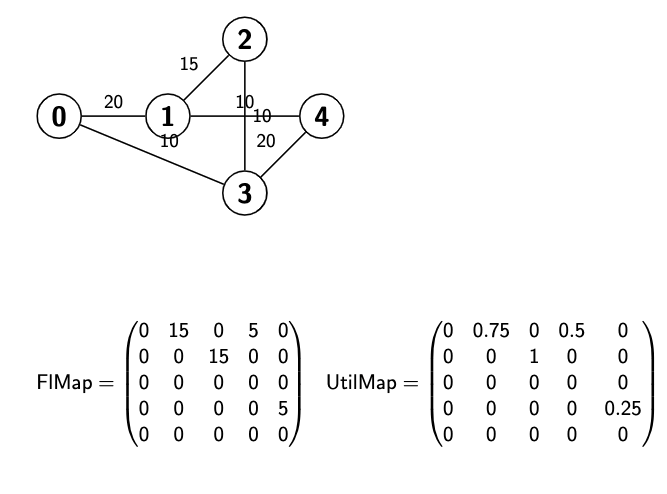
\includegraphics[width=\linewidth]{figures/2.png}
\caption{Topologie für die Tests des Algorithmus Erweiterte DemandsFirstWaypoints }
\label{fig2}
\end{figure}

\begin{figure}
\centering
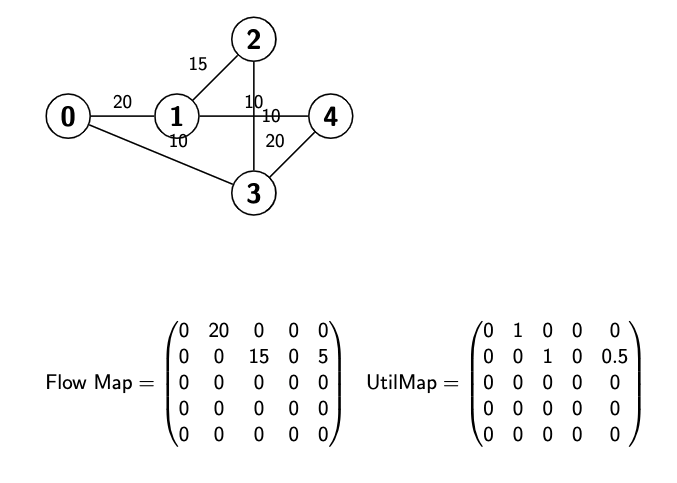
\includegraphics[width=\linewidth]{figures/3.png}
\caption{Topologie für die Tests des Algorithmus Erweiterte DemandsFirstWaypoints }
\label{fig3}
\end{figure}

Resultate: In Abbildung \ref{fig4} wird eine grafische Darstellung der Ergebnisse von newWeights (in blau) und dfw (in rot) präsentiert. Hierbei lassen sich die beiden Verläufe direkt miteinander vergleichen, da sie für dieselbe Topologie und dieselben Anforderungen simuliert wurden.Für dfw sind die initial gewichte auf 1 gesetzt, und Knoten 1 dient als Zwischenstation für die Nachfrage (0->2,15), während Knoten 3 als Zwischenstation für die Nachfrage (0->4,5) fungiert.In Abbildung \ref{fig2} ist die manuell berechnete "util-map" zu sehen.\\
Im Fall von newWeights werden unterschiedliche Gewichtungen verwendet, wobei Knoten 1 als Zwischenstation für beide Anfragen dient.\\
Insgesamt würden die Ergebnisse zwischen den beiden Fällen variieren, abhängig von den Gewichtungen der Kanten. Im Fall von gleichen Gewichtungen könnten die Ergebnisse ähnlich sein, während bei unterschiedlichen Gewichtungen die Wahl der Zwischenstation und der Pfade unterschiedlich sein könnte.

\begin{figure}
\centering
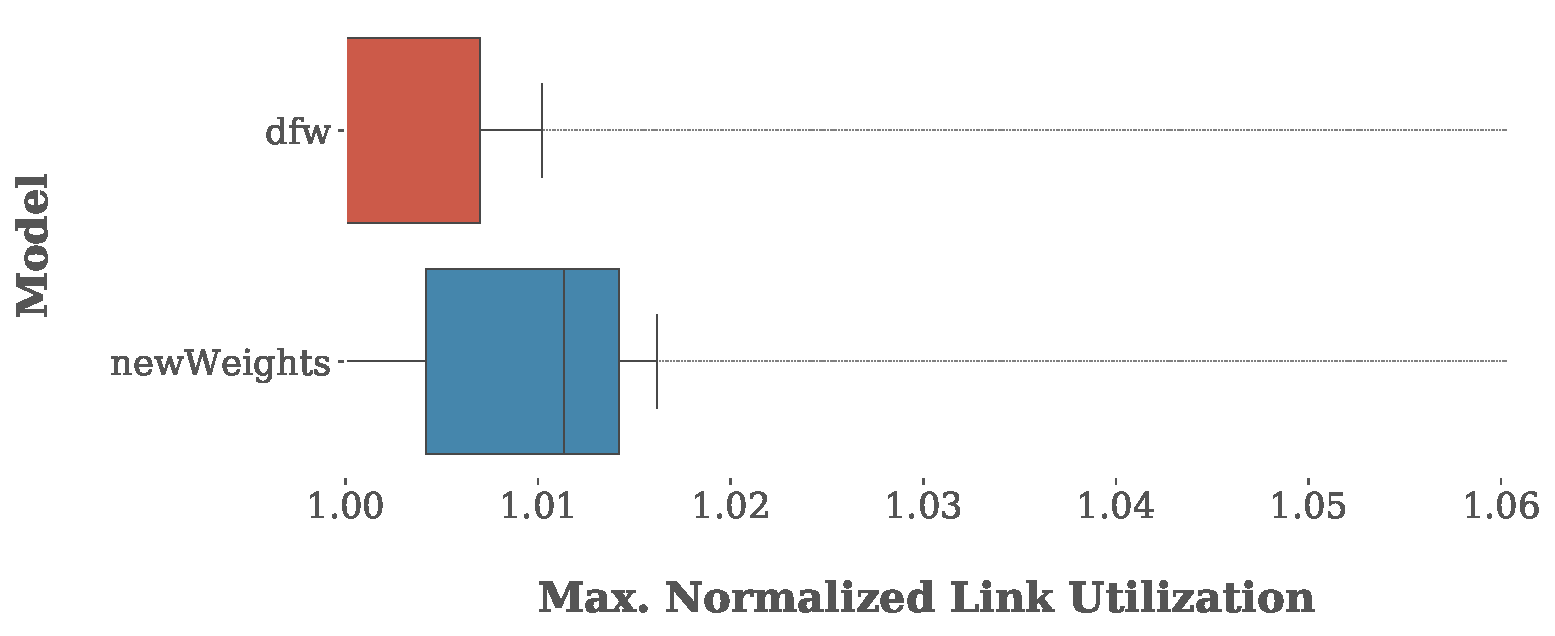
\includegraphics[width=\linewidth]{figures/batch_result001.pdf}
\caption{Ergebnisse für die Tests des Algorithmus Erweiterte DemandsFirstWaypoints }
\label{fig4}
\end{figure}

In diesem speziellen Szenario, wie in Abbildung \ref{fig5} dargestellt, gibt es zwei potenziell kürzeste Wege von A nach D: A -> B -> D und A -> C -> E -> D. Die Methode würde überprüfen, ob das Einfügen eines Wegpunkts auf einem dieser Wege die maximale Auslastung reduziert.\\
Basierend auf der maximalen Auslastung und den Kapazitäten der Kanten könnte sie dann entscheiden, wie die Anforderungen am effizientesten aufgeteilt werden können, um die Auslastung zu optimieren.\\
Mehrere kürzeste Pfade, unterschiedliche Anforderungen, Kapazitätsbeschränkungen und Effizienz könnten den Algorithmus vor besondere Herausforderungen stellen. Der Algorithmus muss eine gründliche Analyse durchführen, um die optimale Verteilung der Anforderungen auf die Pfade zu finden und gleichzeitig die Kapazitätsbeschränkungen zu berücksichtigen, wie in Abbildung \ref{fig5} dargestellt.

\begin{figure}
\centering
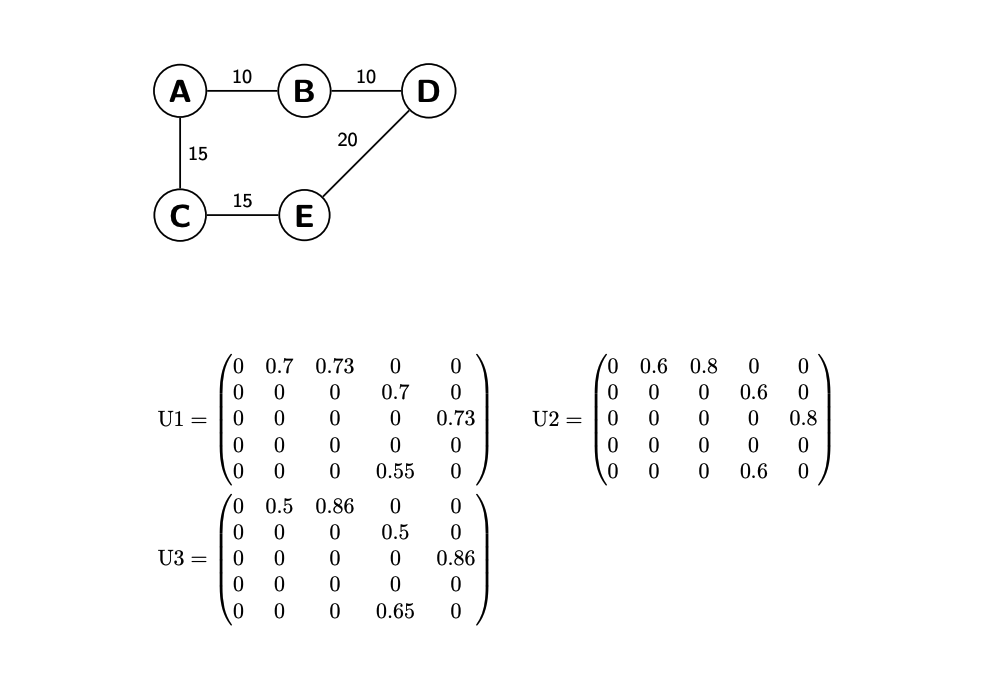
\includegraphics[width=\linewidth]{figures/1.png}
\caption{Topologie für die Tests des Algorithmus Erweiterte DemandsFirstWaypoints }
\label{fig5}
\end{figure}




\section{Zusammenfassung}
Die Ergebnisse dieser Arbeit trugen nicht nur zum akademischen Diskurs bei, sondern lieferten auch praktische Erkenntnisse von großer Bedeutung für die Netzwerktechnologie. Durch die Analyse der Auswirkungen der kombinierten Optimierung von Linkgewichten und Wegpunkten auf die Netzwerkleistung wurden wertvolle Einblicke gewonnen. Diese Erkenntnisse haben das Verständnis dafür vertieft, wie Netzwerke effizient gestaltet werden können, um den Datenverkehr unter Berücksichtigung von Engpässen und Prioritäten optimal zu lenken. Solche Erkenntnisse sind von direktem Nutzen für Netzwerkingenieure, IT-Experten und Unternehmen, die eine zuverlässige und leistungsfähige Kommunikationsinfrastruktur benötigen.\\
Darüber hinaus bot das Projekt den teilnehmenden Studierenden eine einzigartige Gelegenheit, praktische Fähigkeiten im Bereich der Netzwerktechnologie zu entwickeln und zu erweitern. Die Konzeption und Implementierung der Routingalgorithmen erforderte nicht nur technisches Know-how, sondern förderte auch die Fähigkeiten in den Bereichen Problemlösung, kreatives Denken und Teamarbeit. Diese praktischen Erfahrungen werden die Studierenden auf ihre zukünftigen Karrierewege vorbereiten, sei es in der Forschung, der Industrie oder im Bereich der Informationstechnologie.\\
Insgesamt hat dieses Fachprojekt nicht nur zur wissenschaftlichen Erkenntnisgewinnung beigetragen, sondern auch dazu, dass die Teilnehmerinnen und Teilnehmer eine echte Verbindung zur praktischen Anwendung von Netzwerktechnologien herstellen konnten. Diese Erfahrung wird nicht nur ihre akademische Laufbahn bereichern, sondern auch dazu beitragen, ihre beruflichen Fähigkeiten in einem Bereich zu schärfen, der zunehmend an Relevanz gewinnt – der Gestaltung und Verwaltung hochleistungsfähiger Netzwerkinfrastrukturen.

\begin{acks}
Herzlicher Dank an Marin f\"ur seine Unterstützung und seine geduldige Begleitung bei der Bewältigung unserer Herausforderungen.
\end{acks}

\bibliographystyle{ACM-Reference-Format}
\bibliography{fapro_bib}

\appendix

\end{document}